\chapter{Introduction} \label{chapter:prelude}

\section{Motivation}

Virus proteins interact with their host's cellular machinery, and in
doing so alter the host cell to favor viral replication. It is
important to identify and annotate virus-host interactions for the
discovery of new drug targets as well as for assessing the efficiency
of antiviral drug therapies on host subpopulations
\cite{brass08,dampier09}. Furthermore, virus-host interactions can be
used to suggest roles for virus proteins \cite{calderwood07}, and
investigate common viral strategies for interacting with their hosts
\cite{navratil-system}. With this in mind, many researchers have
gathered data for virus-human interactions to determine host factors
necessary for the virus life cycle. These interactions take the form
of virus-human protein interactions, human gene expression responses
to infection, and genetic screens for human genes that are necessary
for virus survival. The genetic screens suggest that certain human
genes play a role in infection, while the protein interaction and gene
expression data suggest what these roles might be. To date, only three
viruses, human immunodeficiency virus (HIV), hepatitis C virus (HCV),
and influenza A virus have extensive data for these interactions.

The experimental challenges of identifying virus-host protein
interactions are numerous. The biggest challenge is designing screens
stringent enough to have low false positive rates while ensuring that
the number of real interactions that cannot pass these stringent
assays is kept to a minimum. Protein interactions are transient in
nature, and moreover such protein binding interactions may depend on
the presence of cofactors that are not necessarily present in binding
assays. These difficulties suggest supplementing experiments with a
bioinformatic approach to predicting and understanding virus-host
interactions. This has been attempted for HIV by predicting HIV-human
protein interactions, but it was found that the most predictive human
protein feature was the number of interacting partners a protein had
\cite{tastan09}, which does not provide sites for drug targeting. Such
findings indicate that more analysis is needed to understand the
underlying principles of interactions, and to guide experimental
studies.

The overall goal of this dissertation is to estimate and analyze
virus-host interactions. These interactions have been organized into
networks, where proteins are nodes and network edges represent
interactions between proteins \cite{han04}. We begin this thesis by
predicting virus-host protein interactions using short peptide motifs
that have been shown to play a role in protein interactions
\cite{kadaveru08}. We demonstrate the validity of our predictions
using HIV-human interactions. Next we investigate the usage of
mitogen-activated kinase docking motifs on HIV proteins. We then
compare HCV, HIV, and influenza virus-host networks to address the
finding that virus proteins prefer to interact with highly connected
host proteins. We provide evidence that this hub preference is a
consequence of the requirement of viruses to utilize host protein
complexes during infection. We conclude this dissertation with a
discussion of how the work presented here aids virus-host network
analysis.

\section{Organization}
This thesis has been organized into three specific aims: (1) the
prediction of virus-host interactions using sequence motifs, (2) the
refinement of virus sequence motifs, and (3) the analysis of virus
targeted host proteins.

This chapter serves as a background section. We will discuss two types
of virus-host interactions: protein interactions gathered from high
throughput studies and literature searches, and siRNA screens
searching for host factors required for the viral life cycle. Next, we
will cover previous studies of virus-host networks, describing network
and gene analysis and the importance of peptide motifs in virus-host
protein interactions. We will then conclude  with a description
of methods for predicting protein interactions, and illustrate how
they have been applied to virus-host interactions.

Chapter \ref{chapter:predict} is devoted to the first aim, the
prediction of virus-host protein interactions, which are important for
guiding experimental studies
\cite{jansen2003bayesian,lee2004probabilistic}. We focus this aim on
interactions between HIV and human proteins and show that a list of
host proteins highly enriched with those targeted by HIV proteins can
be obtained by searching for host protein motifs along virus protein
sequences. We find that peptide motifs conserved across 70\% of HIV
protein sequence samples occur in similar positions on HIV proteins,
and we document protein domains that interact with these conserved
motifs. We predict which human proteins may be targeted by HIV by
taking pairs of human proteins that may interact via a peptide motif
conserved in HIV and the corresponding interacting protein domain. Our
predictions are enriched with host proteins known to interact with HIV
proteins Env, Nef, and Tat (p-value $<$ 4.26e-21). Cellular pathways
statistically enriched for our predictions include the T-cell receptor
signaling, natural killer cell mediated cytotoxicity, cell cycle, and
apoptosis pathways. Molecular functions enriched with both predicted
and confirmed HIV targeted proteins include phosphorylation and adenyl
ribonucleotide binding. This study validates the role of peptide
binding motifs in guiding virus-host interactions and suggests new HIV
targeted pathways and proteins in the host cell.

In Chapter \ref{chapter:mapk} we discuss the second aim, the
refinement of virus motifs. Over the course of HIV infection, virus
replication is facilitated by the phosphorylation of HIV proteins by
human ERK1 and ERK2 mitogen-activated protein kinases (MAPKs). MAPKs
are known to phosphorylate their substrates by first binding with them
at a consensus docking site motif. Docking site interactions could be
viable drug targets because the sequences guiding them are more
specific than phosphorylation consensus sites. In this study we use
multiple bioinformatics tools to discover candidate MAPK docking site
motifs on HIV proteins known to be phosphorylated by MAPKs, and we
discuss the possibility of targeting docking sites with drugs. Using
alignments of multiple HIV protein sequences taken from different
patients, we show that the consensus MAPK docking pattern previously
described for human proteins is missing from a significant fraction of
the sequences gathered for HIV proteins known to be phosphorylated by
ERK1 and ERK2. We revise the consensus MAPK docking pattern in order
to provide patterns that annotate that the majority of sequences for
all HIV proteins. One revision is based on a documented human variant
of one of the consensus MAPK docking motif, and the other reduces the
number of required basic amino acids in the consensus docking motif
from two to one. The proposed patterns are shown to be consistent with
in silico docking between ERK1 and the HIV matrix protein. The motif
usage on HIV proteins is sufficiently different from human proteins in
amino acid sequence similarity to allow for HIV specific targeting
using small-molecule drugs. 

We tackle the third aim, the analysis of virus targeted highly
connected human proteins, in Chapter \ref{chapter:hubs}. HIV,
influenza virus, and other human viruses preferentially interact with
highly connected proteins, or hubs, in the human protein interaction
network \cite{calderwood07, dyer08, dechassey08, tastan09}. Hub
proteins have been classified into two groups by co-expression with
their interacting neighbors \cite{taylor09}. Intermodular, or date,
hubs are defined as being co-expressed with their neighbors in certain
tissues, while intramodular, or party, hubs are characterized by
co-expression with their neighbors in most tissues
\cite{taylor09}. The existence of these two hub classes is under
debate \cite{taylor09,batada06,batada07,agarwal09,han04}. Here we
provide new evidence for this hub distinction, and ask if hub proteins
that interact with virus proteins have a hub class preference. For HIV
and influenza virus, we show that hubs that directly interact with a
virus protein are more likely to be intramodular than
intermodular. This preference is important because the features of
intramodular hubs that are different from intermodular hubs serve as
hypotheses for features that virus proteins target in host
proteins. The virus intramodular hub preference is also important for
the study of biological networks because it is further evidence for the
existence of two hub classes.

The thesis concludes in Chapter \ref{chapter:conclusion} with a review
of the material presented and a discussion of future work for
virus-host interactions. We will summarize our major discoveries and
testable hypothesis generated in Chapters \ref{chapter:predict},
\ref{chapter:mapk}, and \ref{chapter:hubs}. Next, we will discuss
future work that stems from this dissertation. We will show how
protein structure and virus-host network patterns can be used jointly
with the peptide motifs from the first aim to arrive at a new set of
virus-host interaction predictions. We will cover how peptide motifs
on virus proteins can be validated by constructing a database of virus
protein mutations and their affects on virus-host interactions, and we
will discuss a project to test the hypothesis that virus proteins
serve as intermodular hubs in virus-host networks. We will also
propose a project to test that hypothesis that influenza virus uses
different versions of peptide motifs based on which host it infects.

\section{Review of virus-host interactions}

\begin{table}\footnotesize
\begin{center}
  \begin{tabular}{|l|c|c|}
  \hline
  Virus & siRNA screen hits & Protein interactions (Interacting human proteins) \\
  \hline
HIV & 850 & 2652 (887) \\
HCV & 318 & 477 (414) \\
Influenza & 295 & 339 (230) \\
Papillomavirus & NA & 229 (94) \\
EBV & NA & 173 \\
KSHV & NA & 173 \\
VZV & NA & 123 \\
\hline
  \end{tabular}
\end{center}
\caption[Experimentally determined virus-host interactions]{\small For
  each virus, we show the number interactions that occur between virus
  and human proteins, and count the number of host factors necessary
  for infection (siRNA screen hits). Of the viruses in the table, HCV,
  HIV, and influenza virus have the most experimentally determined
  virus-host interactions. siRNA screen hits describe interactions
  between a virus and a human gene. siRNA screens have only been
  conducted for HCV, HIV, and the influenza virus. Protein
  interactions cover only direct interactions, like protein binding or
  protein modifications, such as the phosphorylation of a virus
  protein by a host kinase. A single human protein can be involved in
  multiple interactions with different virus proteins, so the total
  number of unique human proteins involved in virus-human interactions
  is given in parentheses. While only direct interactions are listed
  here, HIV has a total of 3950 direct and indirect (e.g. regulatory,
  induced protein modification) interactions with 1439 human proteins
  \cite{fu09}. \label{tbl:intro:counts}}
\end{table}


While single species protein-protein interaction networks have been
gathered in high throughput screens and studied for ten years,
virus-host networks are only recently the subject of investigation
\cite{mendez2010global}. Large scale studies of virus-host
interactions have focused on HIV, HCV, and the influenza virus.
Smaller studies have been conducted for Epstein-Barr virus (EBV)
\cite{calderwood07}, Kaposi sarcoma-associated herpesvirus (KSHV),
Varicella-Zoster virus (VZV) \cite{uetz2006herpesviral}, and
Papillomavirus \cite{driscoll2009pig}. Virus-host interaction data
have primarily been collected from small interfering RNA (siRNA)
screens, high throughput binding assays, and literature reviews. siRNA
screens were performed in infected cells to find host factors that
could be knocked down without harmful effects on the host, but would
inhibit virus replication \cite{georgel2010virus}. Table
\ref{tbl:intro:counts} enumerates virus-host interactions gathered for
different viruses.

%Binding assays ...

%Literature reviews ... 

We focus on HIV, HCV, and influenza virus for two reasons. First,
unlike EBV, VZV, and KSHV, all three viruses have small proteomes,
making them more reliant on host cell machinery during their life
cycles. Second, the interactions of HCV, HIV, and influenza virus with
human proteins are well studied, and include both protein interactions
and siRNA data. The following section describes the interactions for
these three viruses in detail, and later we discuss principal findings
from previous studies of these networks, and initial attempts to model
them.

\subsection{Datasets}

\subsubsection{HIV-human interactions}

\begin{figure}
\begin{center}
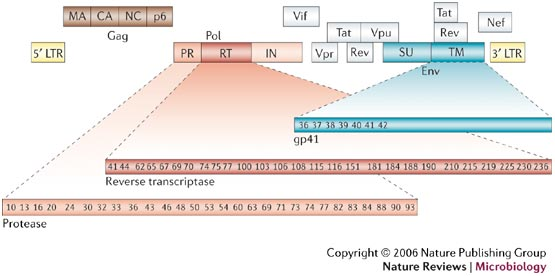
\includegraphics[scale=0.75]{figs/hiv_proteins}
\end{center}
\caption[HIV genome]{\small HIV contains nine open reading frames and
  produces around twenty proteins. This image was taken from an HIV
  review article \cite{lengauer2006bioinformatics}. Permission to
  reuse this figure was granted by the publisher, copyright 2006
  Nature Publishing Group. \label{fig:hiv_proteins}}
\end{figure}

HIV is an RNA virus of roughly nine kilobases encoding nine open reading
frames that produce around twenty proteins (Figure
\ref{fig:hiv_proteins}) \cite{frankel2003hiv}. There are different
subtypes, or strains, of HIV, and these are classified hierarchically,
starting with three groups: major (M), outlier (O), and non-major and
non-outlier (N) \cite{taylor08}. Group M, which is the most common,
has been divided into nine subtypes, or clades: A, B, C, D, F, G, H, J
and K. Sequences from the same subtype are more similar to each other
than to sequences in other subtypes. Some subtypes correspond to
geographical locations. Recombinant forms of group M subtypes have
been identified. For instance, 01\_AE is a combination of subtypes A
and E that is circulating in Southeast Asia \cite{taylor08}. Subtype E
has not been found in a non recombinant form, so it is not listed in
the nine subtypes of group M. Five subtypes and two recombinants are
present in at least 2.5\% of the world population \cite{taylor08}.

Interactions between human proteins and HIV proteins come mostly from
literature curation rather than high throughput binding
assays. Interactions between HIV and human proteins have been
cataloged in VirusMINT \cite{chatr08} the NCBI HIV-Human Protein
Interaction Database \cite{ptak08}, and the pathogen interaction
gateway (PIG) \cite{driscoll2009pig}. From these databases, it has
been observed that HIV proteins interact with many of the same host
proteins \cite{fu09}. HIV-human interactions come in two types, direct
and indirect. Direct interactions involve physical protein contact,
and include binding interactions, protein modifications, and cleavage
interactions. Indirect interactions involve gene expression regulation
and indirect effects, such as inducing protein modifications or
cleavage. In HIV-human interaction databases, the number of human
proteins involved in indirect virus-host interactions is roughly twice
the number that are involved in direct interactions \cite{fu09}.

Not all of these interactions will occur \textit{in-vivo}, or be relevant to
HIV infection. Direct interactions pertinent to infection can be found
by comparing these protein interaction databases to siRNA screens for
host factors involved in HIV replication. Four large such screens,
each resulting in around two hundred host factors have been conducted
for HIV \cite{zhou08, konig08, brass08, yeung09}. There was little
overlap between the four screens \cite{yeung09, bushman09}. While this
might be attributed to differences between the cell types used, more
than 90\% of the genes deemed important for HIV infection were
expressed in all cell types \cite{bushman09}. Other explanations for
different results include experimental error, different filtering
thresholds for deciding which host genes resulted in cell lethality
when knocked down, and differences in the infection time points
analyzed \cite{bushman09}.

%% This is a trend
%% seen not only for HIV, but for HCV as well.

\subsubsection{HCV-human interactions}

\begin{figure}
\begin{center}
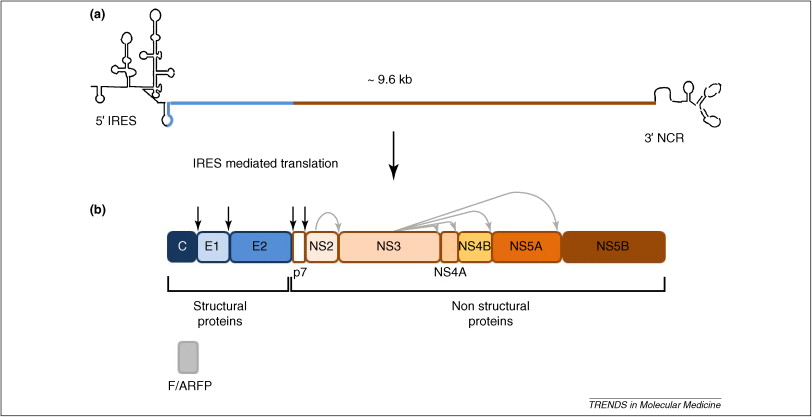
\includegraphics[scale=0.75]{figs/hcv_proteins}
\end{center}
\caption[HCV genome]{\small (a) HCV genome and (b) HCV
  polyprotein. This image was taken from a review of HCV-human
  interactions \cite{georgel2010virus}. Permission to reuse this
  figure was granted by the publisher, copyright 2010 Elsevier
  Ltd. \label{fig:hcv_proteins}}
\end{figure}

HCV is a 9.6 kb positive-strand RNA virus that encodes a 3000 residue
polyprotein, which is cleaved by host and virus proteases into ten
proteins (Figure \ref{fig:hcv_proteins})
\cite{moradpour2007replication}. Chronic HCV infection leads to
serious liver disease \cite{georgel2010virus}, with roughly three
percent of the world's population infected
\cite{shepard2005global}. In the last decade, several infectious model
systems have enabled the accumulation of HCV-human interactions
\cite{georgel2010virus}.

The HCV-human protein interaction network has been constructed from
high-throughput screens augmented with a literature curation
\cite{dechassey08}. Unlike HIV, there is little overlap between the
host binding partners of HCV proteins, and all HCV-human interactions
are for direct protein binding. Several small siRNA screens have been
combined with a larger genome-wide screen to arrive at over three
hundred host factors required for HCV infection \cite{Li09}. While the
HIV genetic screens focused on host dependency factors, some HCV siRNA
screens looked for host factors that when knocked down caused an
increase in virus replication. These were likely host genes that were
part of the immune response. One such screen identified twenty five
such genes \cite{Li09}.

\subsubsection{Influenza-human interactions}

Influenza A virus is a negative-strand RNA virus that encodes eleven
proteins using eight individual RNA segments
\cite{clancy2008genetics}.  An early influenza virus siRNA screen,
conducted in fly rather than human cells, identified 100 fly genes
involved in influenza virus replication \cite{hao2008drosophila}. Two
recent studies have tried to pin down the human pathways and genes
involved in influenza A infection. A genome-wide siRNA screen in cells
infected with influenza A virus identified 295 host factors required
for influenza replication \cite{konig2009human}. A more detailed study
extensively cataloged three types of interactions between host and
virus: protein-protein, host gene expression response, and siRNA
screens \cite{shapira2009physical}. Like the HCV siRNA data, this
study looked at both positive and negative virus response to host
knock down, providing lists of necessary host factors and possible
immune response genes. Analysis of the data revealed many aspects of
the host immune system to interact with the virus.

\section{Previous work with virus-host interactions}

It is important to study and model virus-host interaction networks at
protein, the pathway, and network levels to understand virus protein
function \cite{calderwood07}, help design antiviral therapies
\cite{brass08,dampier09}, guide virus-host protein interaction
experiments \cite{jansen2003bayesian,lee2004probabilistic}, and
compare the ways in which viruses alter host cellular pathways
\cite{navratil-system}. Each interaction abstraction has yielded
important insights. Protein level studies often describe binding site
on both virus and host proteins. Pathway level studies have revealed
subsets of human proteins that are likely to interact with virus
proteins. These studies can be used as a guide for more detailed
experiments as the protein level, and to compare virus-host protein
integrations in terms of biological processes instead of individual
proteins. Network level studies have allowed viruses to be compared to
find trends common to infection.

%% ... Virus-host interactions have been studied at the protein level,
%% the pathway level, and the network level. Each interaction abstraction
%% has yielded important insights. Protein level studies often describe
%% binding sites on both virus and host proteins, while pathway and
%% network level studies allow viruses to be compared to find trends
%% common to infection. 

\subsubsection{Protein studies}

At the protein level, studying the binding regions on virus and human
proteins will aid in finding small-molecule drugs to prevent
virus-host interactions. A recent study produced a number of
U.S.\ Food and Drug Administration approved small-molecule drugs that
could inhibit certain protein interactions after screening these drugs
for their ability to disrupt protein complexes with known peptide
binding sites and available 3D structures
\cite{parthasarathi2008approved}. Without knowledge of the protein
binding sites, this study would not have been possible.

The bulk of HIV protein interactions has come from collections of
single protein studies \cite{mendez2010global, chatr08, ptak08,
  driscoll2009pig}. In addition to helping to build the HIV-human
protein interaction network, these individual interaction studies have
given insights into how virus-host interactions occur. It is now
proposed that binding between host and virus proteins occurs between
short peptide motifs on virus proteins, and protein domains on human
proteins \cite{tonikian08,shelton08,kadaveru08}. Figure
\ref{fig:intro:nef} shows some motifs on the HIV NEF protein. Each
motif is associated with a domain or set of proteins that interact
with it. A database of host peptide motifs and the domains that
interact with them exists at the Eukaryotic Linear Motif (ELM)
Resource \cite{puntervoll03}. The ELM Resource has cataloged over 130
of these peptide motifs and constructed a pattern that matches each
one using documented motif instances from the literature.  Work with
binding regions on virus and host proteins has been hampered by a
disconnect between the eukaryotic work done with peptide motifs and
the study of virus-host interactions. In this dissertation, we combine
knowledge from the ELM Resource with virus-host protein interactions
to study the ability of peptide motifs to explain interactions between
virus and host proteins.

\begin{figure}
\begin{center}
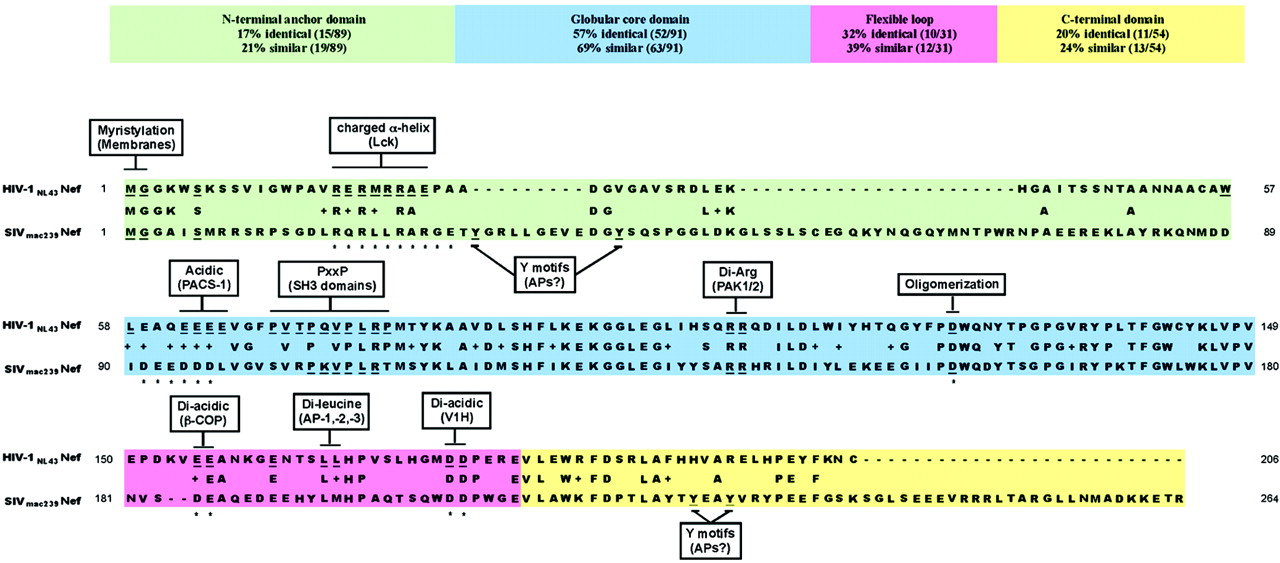
\includegraphics[scale=0.25]{figs/intro_nef}
\end{center}
\caption[Host peptide motifs on HIV NEF]{\small HIV and SIV NEF harbor
  short peptide motifs that enable them to interact with host cell
  proteins and alter host trafficking. This image was taken from a
  review of the affects of NEF on host cell trafficking
  \cite{roeth06}. Permission to reuse this figure was granted by the
  publisher, copyright 2006 American Society for
  Microbiology. \label{fig:intro:nef}}
\end{figure}

\subsubsection{Pathway studies}

Knowledge of which host cellular pathways are targeted by viruses
helps to narrow the focus of experiments determining virus-host
protein-protein interactions \cite{lee2004probabilistic}. Experimental
methods for determining protein interactions are costly and require
much time and effort, so methods to guide experiments are desirable
\cite{skrabanek2008computational}. Mapping the yeast interaction
network required several high throughput yeast two-hybrid screens due
to the false negative rates of these assays
\cite{collins2007toward,huang2009precision}. Focusing on specific
pathways important for infection will reduce the cost and time
required for such experiments.

Pathways are also useful for comparing viruses, or multiple siRNA
screens investigating host factors required by a virus. Comparing HIV
siRNA screens at the gene level showed little overlap between results,
but at the pathway level results became more consistent
\cite{yeung09}. Some common HIV targeted pathways included NF$\kappa$B
signaling, estrogen-receptor signaling, peroxisome
proliferator-activated receptor signaling, RAR activation, and caspase
apoptosis routes \cite{yeung09}. Similarly, pathway analysis of siRNA
screens in HCV and other Flaviviridae virus identified TGF$\beta$,
ErbB, MAPK, focal adhesion, and ubiquitin-mediated proteolysis as
common Flaviviridae virus pathways \cite{Li09}. Influenza virus, HIV,
EBV, and KSHV, have also been found to target similar immune response
pathways \cite{shapira2009physical,brander2000modulation}.

Pathway studies have also facilitated the annotation of virus proteins
of unknown function \cite{calderwood07}, and the comparison of viral
strategies for subverting the human type I interferon response
\cite{navratil-system}. Investigations of virus targeted pathways have
led to hypotheses concerning virus protein function. Analyzing the
pathways that were found to interact with Epstein-Barr virus (EBV)
proteins allowed investigators to infer roles for unannotated EBV
proteins \cite{calderwood07}. Another pathway study of virus protein
interactions with host proteins involved in the human type I
interferon response revealed that virus proteins from four viral
families (Flaviviridae, Herpesviridae, Papillomaviridae, and
Retroviridae) targeted different aspects of the response, which
consists of a four level cascade of interactions traveling from host
receptors, to adapters and mediators, and ending at transcription
factors that initiate the immune response
\cite{navratil-system}. Viruses in the Flaviviridae and Herpesviridae
families targeted host proteins with many host interactions in the
interferon pathway, focusing on protein adapters, mediators, and
transcription factors. Viruses in the Retroviridae and
Papillomaviridae families mostly targeted transcription factors.

One issue holding back pathway level studies is the availability of
experimental data. High throughput yeast two-hybrid and siRNA screens
have only been conducted for a handful of viruses. It would be nice to
compare viruses without such datasets by only using sequence
information, which is becoming easier to gather
\cite{munroe2010third}. In this dissertation, we address this problem
by describing a way to use peptide motifs on virus proteins to predict
virus targeted pathways.

%% Virus-host protein interactions or RNAi screen results can be used to
%% find enriched pathways. Pathways found to be enriched with HCV
%% interacting host proteins were insulin, TGF$\beta$, Jak/STAT, and
%% focal adhesion \cite{dechassey08}.  Influenza virus interacting proteins proteins were found
%% to interface significantly with p53, PML, TNFR/Fas-mediated apoptosis,
%% NF$\kappa$B, and WNT pathways
%% \cite{shapira2009physical}. Interestingly, the WNT pathway has been
%% implicated in immune response \cite{staal2008wnt}, indicating that
%% some virus-host PPIs target the immune system. A second influenza RNAi screen found
%% trafficking pathways, actin organization, MAPK, proteases,
%% ubiquitination, calcium signaling, and the AKT pathway to be involved
%% in early steps of virus replication \cite{konig2009human}.

\subsubsection{Network studies}

While these pathway level studies are important, to understand
infection as a system, researchers began investigating the virus-host
interaction network. One network based analysis of virus-host networks
searched for network motifs in the HIV-human interaction network
\cite{hivNetMotifs}. Network motifs are statistically over-represented
interaction patterns in networks. An example is a feed back loop in a
regulatory network, where a gene controls the expression of its
regulator. Network motifs have been identified in yeast protein
interaction networks \cite{wuchty2003evolutionary}, E. coli
transcriptional regulation networks \cite{shen2002network}, and
synthetic genetic interaction networks \cite{costanzo2010genetic}. In
an initial study of cross-species network motifs, the HIV-human
network was searched for motifs that might aid the virus in taking
control of the host cell.

Virus-host networks have also been used to achieve a more biological
understanding of interactions. A combined study of HIV siRNA screens
and the host protein interaction network clustered the virus targeted
host network into dense network neighbor hoods. Analysis revealed
these neighborhoods to represent proteasome, mediator, RNA binding and
splicing, and chaperone network components \cite{bushman09}. With a
similar goal in mind, an influenza virus-host network that included
virus-host protein interactions, siRNA screen results, and host
expression response to infection was analyzed to determine which
interactions could be attributed to the host immune system
\cite{shapira2009physical}.

In a study of the network properties of pathogen targeted proteins it
was determined that pathogens like HIV and EBV have proteins that
prefer to interact with human proteins with specific network
properties. Hub proteins and bottleneck proteins, i.e.\ proteins that
separate large components of the host interaction network, were found
to be preferentially targeted by pathogen proteins \cite{dyer08}. A
later topological analysis of the HCV-human interaction network
revealed that HCV proteins also preferred to interact with human hub
and bottleneck proteins \cite{dechassey08}. It has been suggested that
hubs are targeted by viruses because hubs provide an efficient way to
rewire the host network to favor virus production
\cite{calderwood07}. In this dissertation, we address the virus hub
preference, and suggest a biological reason behind it.

%% The best system level study has been
%% conducted for the influenza A virus
%% \cite{shapira2009physical}. Influenza virus proteins interact with
%% significantly more host proteins than expected from the human PPI
%% network, and some human proteins interact with more influenza proteins
%% than expected by chance \cite{shapira2009physical}.

\subsection{Modeling virus-host interactions}

Just as single species protein interaction networks inspired methods
to predict protein interactions, host-pathogen networks have initiated
the search for network and protein features that model and predict
virus-host protein interactions. One study examined HIV-human
interactions to determine what properties, or features, of human
proteins made them more likely to interact with virus proteins
\cite{tastan09}. The features examined included Gene Ontology labels
\cite{ashburner00}, global gene expression profiles, human interaction
partners, human protein domains, and HIV protein motifs, but it was
determined that the most predictive feature was host protein degree,
i.e.\ the number of host proteins that interact with a candidate host
protein. This finding was consistent with other work done with viruses
and host hub proteins, but had the unfortunate effect of predicting
that all viruses will interact with the same host proteins. Another
HIV-human protein interaction prediction method used structural
similarity between host and virus proteins
\cite{doolittle2010structural}. For each HIV protein with an available
structure, the most structurally similar host proteins were found. The
protein interaction neighbors of these host proteins were predicted to
bind to HIV proteins. This method is limited to virus proteins with
determined structures, and virus protein structures are hard to
predict because so many of them are unstructured proteins
\cite{tokuriki2009viral}, so a sequence based approach is preferable.

The work presented in this dissertation continues the exploration of
virus-host interactions at the protein, pathway, and network
level. First, we examine conserved host peptide motifs on HIV
proteins. We show that these motifs can be used to predict HIV-human
interactions, and we make an argument that some motifs should be
refined. Then we seek an explanation for the observation that virus
proteins target host hub proteins.


%% The largest is the National Institute of Allergy and Infectious
%% Diseases (NIAID) HIV, human protein interaction database, which
%% contains roughly 4000 literature curated interactions between human
%% proteins and HIV proteins. Smaller sets of interactions are known
%% between other viruses and the human proteome, but with the exception
%% of HCV (around 300 interactions) and influenza A, there are too few
%% interactions to draw conclusions about common themes across
%% host-pathogen networks.

